\documentclass[sigplan,screen,review,anonymous]{acmart}

\settopmatter{printfolios=false}
\renewcommand{\shortauthors}{Anonymous Author(s)}
\citestyle{acmnumeric}

\usepackage{amsmath}
\usepackage{array}
\usepackage{booktabs}
\usepackage{graphicx}
\usepackage{multirow}
\usepackage{xspace}
\usepackage{xcolor}
\usepackage{enumitem}
\usepackage{pgfplots}
\usepackage{placeins}
\usepackage{hyperref}
\usetikzlibrary{positioning,arrows.meta,fit,calc,backgrounds,patterns}

\pgfplotsset{compat=1.18}

\graphicspath{{img/}}

\newcommand{\system}{\textsc{VeriEdge}\xspace}

\newcommand{\workflowstep}[1]{%
	\tikz[baseline=(n.base)]{
		\node[circle,fill=black,text=white,inner sep=0pt,
		minimum size=0.95em,font=\scriptsize\bfseries] (n) {#1};
	}%
}


\begin{document}

\title{\system: Verifiability-Constrained Placement for Heterogeneous Edge LLM Inference}

\author{Anonymous Author(s)}
\affiliation{
  \institution{Anonymous Institution(s)}
  \country{}
}

\begin{abstract}
	Heterogeneous edge LLM inference is often framed as a resource-placement
	problem: discover idle devices, split a model, and execute. We argue that
	dependable edge inference must additionally treat verifiability as a
	placement constraint. A placement determines not only latency and capacity,
	but also who receives task access, which device/backend mix produces
	shard-boundary states, and whether a disputed execution can be adjudicated
	under bounded evidence.
	We present \system, a verifiability-constrained placement framework for
	heterogeneous edge LLM inference. Before disclosure, \system admits a
	candidate group, shard map, and verifier mode only if measured targets for
	false disputes, tamper detection, sketch size, and challenge cost are
	satisfied. It then commits this decision before access release, so the same
	record governs selective task access, boundary evidence, challenge
	localization, settlement, and future placement history. The verifier profile
	comes from a Tolerance-aware Sketch Tensor Chain (TSTC), which compares
	compact shard-boundary sketches under calibrated drift while preserving
	first-mismatch localization.
	Our prototype combines selective delivery with a controlled sharded-inference
	verification harness. Strict tensor hashing is unusable under honest
heterogeneous execution, while TSTC profiles expose which
device/backend/sketch profile keys are low-risk, high-risk, or inadjudicable.
	In placement replay, risk-constrained placement removes infeasible usage and
	adaptive verifier selection preserves nearly the same queued-workload
	goodput as the network-aware baseline while lowering false-dispute risk.
	In a 100MB selective-delivery
	microbenchmark, placement-defined disclosure reduces median distribution
	latency by 74.8\% on LAN and 81.1\% on WAN at eight selected providers
	relative to replicated encrypted delivery. \system does not provide a universal semantic correctness proof;
	it exposes measured, policy-scoped arbitration evidence before placement.
\end{abstract}

\ccsdesc[500]{Computer systems organization~Dependable and fault-tolerant systems}
\ccsdesc[300]{Security and privacy~Distributed systems security}
\ccsdesc[300]{Software and its engineering~Distributed systems organizing principles}
\ccsdesc[300]{Networks~Peer-to-peer networks}

\keywords{edge AI, decentralized inference, heterogeneous systems, verification, orchestration}

\acmConference[EuroSys '27]{European Conference on Computer Systems}{April 19--23, 2027}{Rabat, Morocco}

\maketitle
\thispagestyle{empty}
\pagestyle{empty}
\raggedbottom

%------------------------------------------------------------
\section{Introduction}
\label{sec:introduction}
%------------------------------------------------------------

Large language models (LLMs) have made high-quality AI inference a
mainstream service~\cite{brown2020language,bender2021dangers}, but the
compute that serves them remains concentrated in centralized clouds. At the
same time, substantial edge capacity sits idle across desktops, laptops,
mobile devices, and small servers~\cite{deng2020edge,meuser2024revisiting}.
Recent decentralized AI systems and prototypes, including EXO, show that
heterogeneous commodity devices can be organized into collaborative
inference clusters~\cite{wang2024sok,exo_github,exo_blog}. These systems
establish an important feasibility point: edge devices can pool resources
for inference. Feasible collaboration, however, is not the same as a
dependable decentralized inference service. A practical service must also
decide who learns the task payload, how heterogeneous execution is audited,
and who can be held responsible when an output is disputed.

Consider a requester that outsources an LLM inference task to a temporary
edge group assembled from heterogeneous devices and backends. If the final
answer looks suspicious, a final-output judge can flag it as
low-quality~\cite{zheng2023judging,liu2025polylink}, but cannot identify
which shard or provider caused the error. A strict checkpoint hash chain can
localize mismatches, but may reject honest executions because heterogeneous
devices, precisions, kernels, and backend stacks do not produce
bitwise-identical intermediate tensors~\cite{goldberg1991floating,
	higham2002accuracy}. Full replay or cryptographic proof generation offers
stronger evidence, but is too expensive for the common path of
large-model inference~\cite{sun2024zkllm,ivanov2025dsperse}. These
tradeoffs expose the central systems problem in decentralized edge LLM
inference: placement is not merely resource allocation. The selected
execution group determines the \emph{data boundary}, because only selected
providers should receive task-access material; the \emph{execution
boundary}, because selected devices and backends define the numerical drift
that honest executions may exhibit; and the \emph{accountability boundary},
because the shard plan determines which provider can be associated with the
first challenged divergence. \textit{Placement is therefore not merely a resource-allocation decision, but the point where resource selection becomes an accountability commitment.}


Prior systems cover only pieces of this problem. Ledger-based computing
resource markets provide identity, escrow, and
settlement~\cite{baranwal2024blockchain,li2023double,habiba2024auction},
but not accountable heterogeneous LLM execution. Judge-based screening is
cheap but weakly attributable~\cite{zheng2023judging,liu2025polylink}.
Verifiable computation and zero-knowledge systems provide stronger evidence,
from ZKML surveys to LLM-specific proof systems~\cite{peng2025survey,
	sun2024zkllm}, but remain too costly for routine edge inference.
Collaborative inference systems demonstrate multi-device or cross-party
execution~\cite{borzunov2023petals,exo_github}, but usually leave task
disclosure and disputes implicit. What is missing is a placement layer that
exposes verifiability before task access is released: a candidate execution
group should be admitted only when its measured device/backend/sketch profile
can satisfy the task's false-dispute, detection, sketch-budget, and
challenge-cost targets.

This paper presents \system, a verifiability-constrained placement framework
for heterogeneous edge LLM inference. \system is built around one principle:
the selected execution group is an accountability boundary. Before task
disclosure, the orchestrator commits the chosen providers, shard map, and
verifier policy. Afterward, the requester publishes one encrypted
task object off chain and releases locator-and-key material only to the
selected group. Normal executions follow a lightweight settlement path.
Disputes escalate to a bounded verifier whose outcome updates settlement and
placement history.

The verifier profile is constructed from a tolerance-aware sketch tensor chain
(TSTC). TSTC treats each checked shard boundary as a checkpoint from which
providers reveal a compact sketch rather than a full tensor. The verifier
compares candidate and reference sketches under tolerances calibrated from
honest heterogeneous runs, then chains checkpoint decisions so that the first
mismatch can be mapped back to a shard boundary. TSTC is parameterized by the
checkpoint sketch: scalar-coordinate TSTC and projected-token TSTC are two
instantiations of the same checkpoint-sketch chain, with the same challenge
protocol but different sketch statistics and comparison rules. TSTC is not a
proof of semantic correctness for every inference; it provides bounded,
localized evidence for the middle ground between cheap output judging and
heavyweight proof systems. This view changes placement: low-cost
verifiability is not a global property of a checker alone, but a measured
property of the model, device/backend pair, shard boundary, sketch budget, and
calibrated tolerance.

We evaluate \system with a coordination prototype, selective delivery, and a
controlled PyTorch shard harness. Selective delivery reduces median
task-distribution latency for 100MB payloads by 74.8\% on LAN and 81.1\% on
WAN at eight selected providers relative to replicated encrypted delivery. In heterogeneous paired
captures across Apple/\allowbreak Metal, BF16, and RTX/\allowbreak FP32
execution stacks, strict tensor hashing rejects every honest heterogeneous
pair. Compact TSTC profiles preserve first-mismatch localization while
exposing which profile keys require stronger sketches or should be avoided.
In placement replay, the network-aware baseline and the risk-constrained
policy illustrate the admission effect: with a fixed projcos4 verifier,
risk-constrained placement reduces infeasible usage from \(1.000\) to
\(0.000\) and lowers expected false-dispute risk from \(0.0105\) to
\(0.0020\), with only a small goodput change. In the queue-aware replay,
adaptive verifier selection removes infeasible usage while preserving nearly
the same goodput as the queue-aware network baseline (\(12.251\) versus
\(12.266\)). The result is not that verification is a universal latency win;
it is that measured verifier profiles change the placement frontier before
task disclosure.

This paper makes the following contributions:
\begin{itemize}[leftmargin=1.5em]
	\item \textbf{Verifiability-constrained placement with accountability.}
	We formulate edge LLM placement as a constrained decision. Before task
	disclosure, the selected group, shard map, and verifier mode must satisfy
	measured targets for false disputes, detection, sketch size, and challenge
	cost. \system commits this decision before access release; the same record
	governs selective task access, boundary evidence, localization, settlement,
	and future placement history.
	
	\item \textbf{TSTC checkpoint-sketch verification.}
	We introduce TSTC, a tolerance-aware checkpoint-sketch chain for
	heterogeneous execution. It compares compact shard-boundary evidence under
	calibrated drift while preserving first-mismatch localization; scalar-coordinate
	and projected-token TSTC are two sketch instantiations of the same challenge
	protocol.
	
	\item \textbf{Measured profiles and closed-loop evidence.}
	We implement a prototype with selective delivery, contract-mediated
	settlement records, and a controlled sharded-inference verification
	harness. Our evaluation constructs verifier profiles from heterogeneous
	checkpoint captures and shows that using these profiles as placement
	constraints removes inadjudicable placements and lowers false-dispute risk
	while preserving useful goodput.
\end{itemize}

%------------------------------------------------------------
\section{System Model and Problem Scope}
\label{sec:model}
%------------------------------------------------------------

This section defines the entities, task objects, trust assumptions, and
placement problem studied by \system. The design mechanisms that implement
this problem formulation appear in Section~\ref{sec:design}. Figure~\ref{fig:system-model}
summarizes the main objects and information flow.

\begin{figure*}[t]
	\centering
	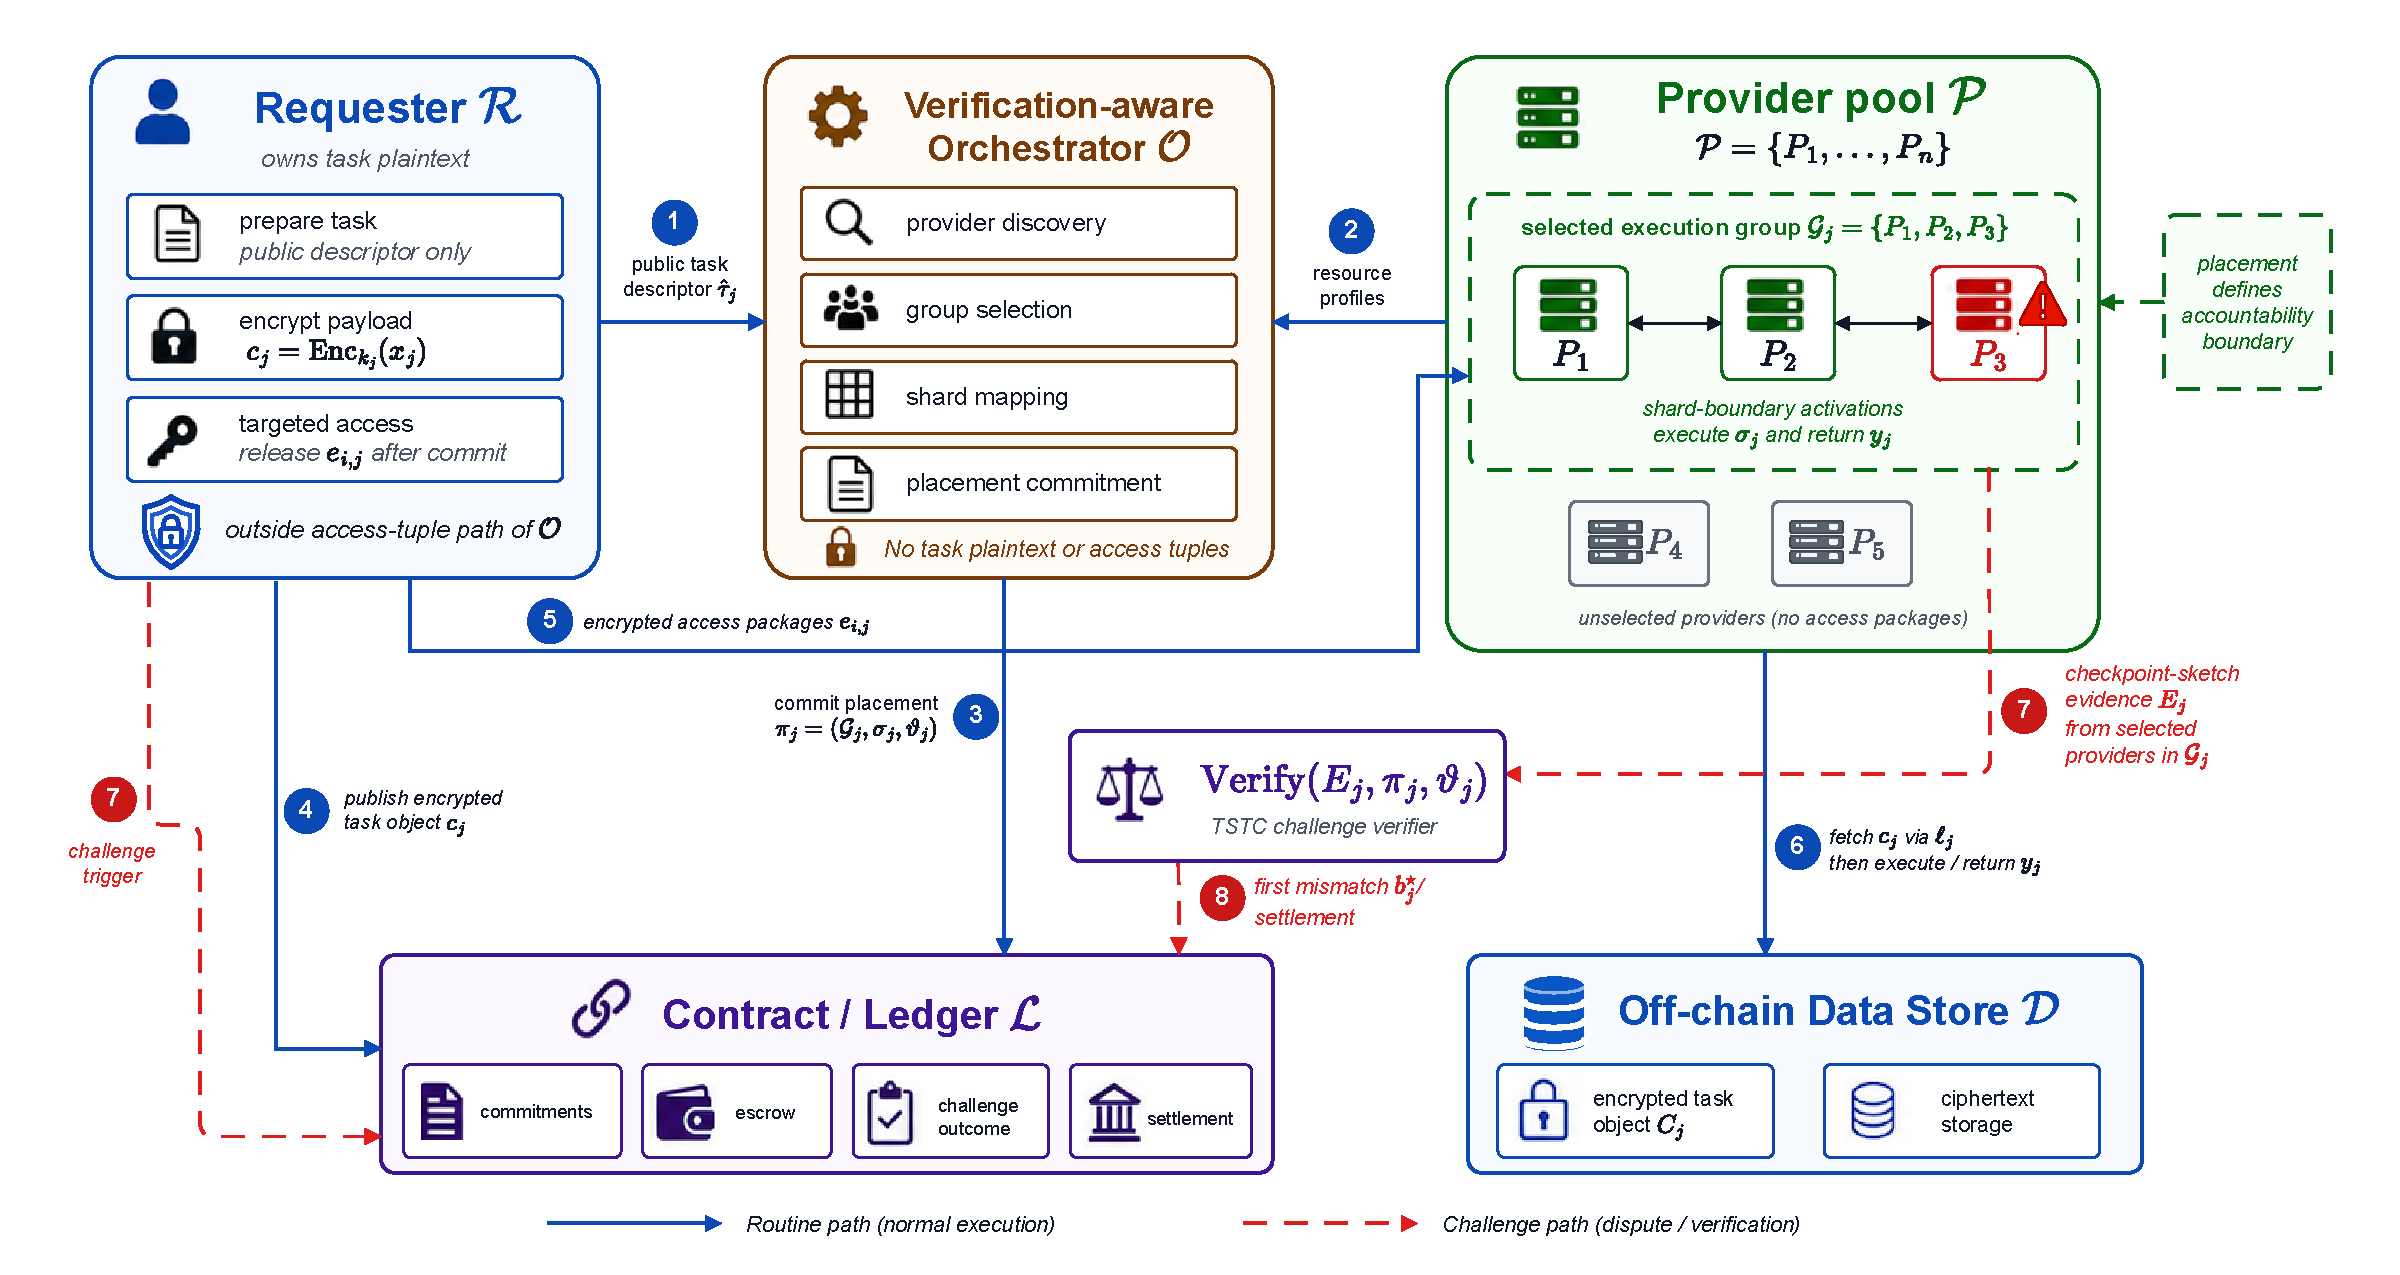
\includegraphics[width=0.9\textwidth]{fig_system_model_workflow.drawio.pdf}
	\caption{\textbf{System model and workflow of \system.}
		The numbered arrows show the eight protocol transitions used by
		\system: public task announcement, provider-profile advertisement,
		placement commitment, ciphertext publication, targeted access release,
		execution, challenge evidence reveal, and verifier/settlement update.
		Section~\ref{subsec:control-loop} groups these transitions into five
		lifecycle phases.}
	\Description{A system model and workflow diagram for VeriEdge. The
		requester sends public task metadata to a verification-aware
		orchestrator, which selects a subset of providers, a shard mapping, and
		a challenge policy, then commits the placement record to a ledger. The
		requester uploads one encrypted task object to off-chain storage and
		sends encrypted locator-and-key access packages only to selected
		providers. Selected providers execute model shards and exchange
		shard-boundary activations; one selected provider is shown as
		potentially faulty under dispute. Unselected providers are shown
		without access packages. A dashed challenge path collects
		checkpoint-sketch evidence, localizes a first mismatching shard
		boundary, and feeds the result to settlement. The orchestrator is shown
		outside the access-tuple disclosure path.}
	\label{fig:system-model}
\end{figure*}

\subsection{Roles and Trust Boundaries}
\label{subsec:entities}

\system considers three active roles: a requester \(\mathcal{R}\), an
orchestrator \(\mathcal{O}\), and a provider pool
\(\mathcal{P}=\{P_1,\ldots,P_n\}\). The requester owns the private task
payload. The orchestrator observes public task descriptors and provider
profiles, selects the execution group, assigns shards, records placement,
and maintains history, but it is not trusted with task plaintext or
per-provider access tuples. Only selected providers receive task access, execute assigned shards, exchange
intermediate activations when collaboration is used, and may reveal
checkpoint-sketch evidence under dispute.


Each provider advertises a public profile \(\phi_i\). The profile contains
coarse resource capacity, network state, device and backend metadata, stake and
reputation state, supported verifier modes, prior challenge history when
available, and a delivery public key \(\mathsf{pk}_i\). These fields are
used for placement admission and ranking; they do not give the orchestrator
access to the requester's private payload.

\system also uses two shared infrastructures. A public ledger
\(\mathcal{L}\) stores compact commitments, challenge state, escrow state,
and settlement outcomes. An off-chain store \(\mathcal{D}\) stores encrypted
task objects and retrievable evidence objects. Neither substrate executes
model computation. The ledger is used for durable coordination and economic
enforcement; ciphertexts, activations, access packages, and sketches remain
off the latency-critical chain path.

\subsection{Task, Placement, and Policy Objects}
\label{subsec:task_model}

\paragraph{Task.}
A private inference task \(j\) is represented as
\(\tau_j=(M_j,x_j,\rho_j)\), where \(M_j\) identifies the model or execution
template, \(x_j\) is the private payload, and \(\rho_j\) is the task policy.
The requester exposes only a public descriptor before placement:
\(\widehat{\tau}_j=(M_j,d_j,\rho^{\mathsf{pub}}_j,\chi_j)\). Here \(d_j\)
is coarse demand metadata, such as a memory or latency class;
\(\rho^{\mathsf{pub}}_j\) is the placement-visible part of the task policy;
and \(\chi_j=\mathsf{Commit}(x_j)\) binds the later encrypted task object to
the private payload without revealing it.

The public task policy includes latency or deadline targets, collaboration
width bounds, disclosure rules, challenge parameters, and the verification
target tuple \((\alpha_j,\beta_j,S^{\max}_j,C^{\max}_j)\). Here
\(\alpha_j\) is the maximum honest false-dispute rate,
\(\beta_j\) is the minimum material-tamper detection rate,
\(S^{\max}_j\) is the sketch/reveal-size budget, and
\(C^{\max}_j\) is the challenge-time verification budget. These targets
make verifiability visible before placement, but they do not reveal
\(x_j\).

\paragraph{Placement.}
Given \(\widehat{\tau}_j\), the model or execution template induces a shard
set \(\mathcal{H}_j\). A placement is
\(\pi_j=(\mathcal{G}_j,\sigma_j)\), where
\(\mathcal{G}_j\subseteq\mathcal{P}\) is the selected provider group and
\(\sigma_j:\mathcal{H}_j\rightarrow\mathcal{G}_j\) assigns each shard to a
selected provider. A single-provider task has one shard; collaborative
inference induces shard boundaries at which providers exchange activations.

In \system, placement is not merely a schedule. The selected group defines
who may later receive task-access material. The shard map defines which
provider is responsible for each model segment and which adjacent provider
pair is associated with each boundary. The combination determines whether a
future dispute can be interpreted through a committed accountability record.

\paragraph{Verification policy.}
A placement candidate is accompanied by a verification policy
\(\vartheta_j=(\mathcal{B}_j,\Phi_j,\mu_j,\Gamma_j,\mathsf{ctx}_j)\). Here
\(\mathcal{B}_j\) is the set of checked shard boundaries,
\(\Phi_j\) is the sketch function, \(\mu_j\) is the comparison rule,
\(\Gamma_j\) is the tolerance map, and \(\mathsf{ctx}_j\) is the seed and
commitment context. The policy specifies compact evidence that a bounded
verifier can request and compare if execution is disputed. It is not a
cryptographic proof system and does not claim semantic correctness for every
possible inference.

\subsection{Threat Model, Goals, and Non-Goals}
\label{subsec:threat}

\paragraph{Adversary and trust assumptions.}
Providers may misreport capabilities, skip computation, deviate from the
shard plan, tamper with boundary states, replay stale evidence, fabricate or
withhold sketches, or return incorrect outputs. Non-selected providers may
try to learn task contents from public metadata or stored ciphertexts.
Collusion within a selected group is in scope for dispute handling, but
\system does not defeat a fully colluding group that produces
self-consistent incorrect execution and evidence. Global Sybil resistance is
outside our contribution except through stake-backed identities and
settlement history.

The orchestrator is trusted to run the advertised coordination logic, but not
with task plaintext or access tuples. Its placement decisions are made
auditable through \(\mathcal{L}\), but \system does not prove that every
placement is globally optimal or strategy-proof. The off-chain store keeps
ciphertexts and evidence objects available, but should not learn task
plaintext without released keys.

\paragraph{Honest heterogeneity.}
Disagreement is not automatically evidence of malice. Honest providers may
produce non-bit-identical intermediate tensors because of floating-point
behavior, precision choices, kernels, hardware, and backend
implementations~\cite{goldberg1991floating,higham2002accuracy}. A useful
dispute mechanism must therefore tolerate benign numerical drift while still
preserving attribution when the evidence supports a material divergence.

\paragraph{Goals.}
Our design pursues five goals:
\begin{enumerate}[leftmargin=1.5em,label=\textbf{G\arabic*:},nosep]
	\item \textbf{Selective disclosure:} only the selected group
	\(\mathcal{G}_j\) receives the locator-and-key material needed to decrypt
	the task payload.
	\item \textbf{Accountable placement:} the same committed placement binds
	task access, shard execution, challenge evidence, and settlement.
	\item \textbf{Drift-tolerant attribution:} verification should tolerate
	benign heterogeneous drift while localizing the first material mismatch
	when the challenged evidence supports it.
	\item \textbf{Verifiability-constrained placement:} hard to adjudicate
	device and backend mixes should be rejected, assigned stronger sketches, or
	charged higher challenge risk before task disclosure.
	\item \textbf{Cheap routine path:} normal executions should avoid
	on-chain optimization, full replay, full-tensor transfer, and heavyweight
	proofs.
\end{enumerate}

\paragraph{Non-goals.}
\system does not provide a cryptographic proof of semantic correctness,
require bitwise-identical heterogeneous execution, design a strategy-proof
resource market, protect model weights from selected providers, place large
tensors on chain, or assume one verifier configuration separates all honest
drift from all tampering. Instead, it targets selective disclosure after
placement commitment, lightweight routine settlement, bounded
checkpoint-sketch challenges, and placement-visible verifiability.

\subsection{Problem Statement: Verifiability-Constrained Placement}
\label{subsec:verifiability-model}

The core problem is to choose, before task disclosure, a provider group,
shard map, and verifier mode. Each candidate must satisfy ordinary resource
constraints and the task's verifiability targets. Low-cost verifiability is
not a global property of a
checker alone. It depends on the model \(M_j\), the selected devices and
backends in \(\mathcal{G}\), the shard assignment \(\sigma\), the checked
boundaries in \(\vartheta\), the sketch statistic, and the calibrated
tolerance.

Thus \system studies the following placement problem: admit and rank only
those heterogeneous placements whose measured verifier profile can satisfy
the task-level false-dispute, tamper-detection, sketch-size, and
challenge-cost targets. A fast device and backend path may be inadmissible if
honest drift repeatedly crosses the selected tolerance. Conversely, a slower
path may be preferable if its checkpoint sketches are stable enough for
cheap adjudication. Section~\ref{subsec:placement} gives the concrete
profile aggregation, feasibility test, and ranking objective used by
\system.




%------------------------------------------------------------
\section{VeriEdge Design}
\label{sec:design}
\label{sec:overview}
\label{sec:orchestration}
%------------------------------------------------------------

\system implements verifiability-constrained placement by tying admission,
task delivery, challenge evidence, and settlement to one committed placement
record. This section describes the mechanisms that enforce that invariant.

\subsection{Design Invariant and Lifecycle}
\label{subsec:overview-invariant}
\label{subsec:control-loop}

For each task \(j\), \system commits
\((\mathcal{G}_j,\sigma_j,\vartheta_j)\) before task disclosure. This
committed tuple is the shared accountability record. It is the data boundary
for task-access release, the execution boundary for shard responsibility,
the evidence boundary for challenged checkpoint sketches, and the settlement
boundary for interpreting localized mismatches.

The numbered arrows in Figure~\ref{fig:system-model} are protocol
transitions rather than independent design modules. For readability, we
describe them in five phases; each phase heading summarizes the following
numbered transitions.

\begin{enumerate}[leftmargin=0pt,label={},labelsep=0pt,itemindent=0pt,nosep]
	\item \textbf{Phase 1: Public announcement and discovery.}
	\workflowstep{1} The requester announces only the public task descriptor
	\(\widehat{\tau}_j\). \workflowstep{2} Providers advertise public resource
	and verification profiles; task-access release occurs later in Phase~3.

	\item \textbf{Phase 2: Verifiability-constrained admission and commitment.}
	\workflowstep{3} The orchestrator enumerates candidate groups, shard maps,
	and verifier modes. It admits only candidates that satisfy resource,
	support, and \((\alpha_j,\beta_j,S^{\max}_j,C^{\max}_j)\) verifier targets.
	The selected
	\((\mathcal{G}_j,\sigma_j,\vartheta_j)\) is then committed in the ledger
	record before disclosure, so later delivery, execution,
	challenge verification, and settlement share one reference record.

	\item \textbf{Phase 3: Selective disclosure and task delivery.}
	\workflowstep{4} After the placement commitment, the requester publishes
	the encrypted task object \(c_j\) to the off-chain data store.
	\workflowstep{5} The requester releases encrypted locator-and-key access
	packages \(e_{i,j}\) only to providers in the committed group
	\(\mathcal{G}_j\). The committed placement is therefore the data boundary:
	unselected providers may observe metadata or ciphertext availability, but
	not the decryption key, and the orchestrator remains outside the
	access-tuple path.

	\item \textbf{Phase 4: Execution and routine settlement path.}
	\workflowstep{6} Selected providers fetch \(c_j\) through the released
	locator, decrypt it with the task key, execute the shard plan
	\(\sigma_j\), exchange shard-boundary activations when collaboration is
	used, and return \(y_j\). Accepted outputs settle on the cheap path without
	full replay, full-tensor transfer, proof generation, or on-chain model
	execution.

	\item \textbf{Phase 5: Challenge verification and feedback.}
	\workflowstep{7} A dispute triggers a challenge; selected providers reveal
	sketch evidence \(E_j\) under the committed verification policy
	\(\vartheta_j\).
	\workflowstep{8} The verifier localizes the first mismatching checked
	boundary \(b^\star_j\) when the evidence exceeds calibrated tolerance,
	maps the result through \(\sigma_j\), and feeds the outcome into
	settlement and future placement history.
\end{enumerate}

This organization separates three planes. The coordination plane records
compact commitments, challenge state, and settlement outcomes; the
execution-and-delivery plane handles ciphertext publication, access-package
delivery, shard execution, and activation exchange; and the verification plane
compares checkpoint sketches only on challenge. The ledger does not store
plaintext, optimize placement on chain, execute model shards, or compare large
tensors.

\subsection{Verifiability-Constrained Placement}
\label{subsec:placement}

For each task \(j\), the orchestrator \(\mathcal{O}\) enumerates candidates
from the public descriptor \(\widehat{\tau}_j\) and provider profiles
\(\{\phi_i\}\). A candidate \((\mathcal{G},\sigma,\vartheta)\) specifies a
selected group, shard map, and verifier mode. It must first pass a hard
admission test before it can be optimized for latency, cost, or reputation.

\paragraph{Measured verifier profiles.}
Calibration runs and prior challenges give the orchestrator a measured profile
for each boundary key. For checked boundary \(b\in\mathcal{B}_j\), let
\(q_{j,b}(\mathcal{G},\sigma,\vartheta)\) denote the profile key induced by
the candidate: the model \(M_j\), boundary \(b\), adjacent execution path
induced by \(\sigma\) and provider profiles, and sketch mode and tolerance
policy specified by \(\vartheta\). A measured profile for key
\(q\) contains four estimates: \(\widehat{\mathrm{FPR}}(q)\),
\(\widehat{\mathrm{TPR}}(q)\), \(\widehat{S}(q)\), and
\(\widehat{C}^{\mathsf{verify}}(q)\): honest false-dispute rate,
material-tamper detection rate, sketch/reveal size, and challenge-time verifier
cost. Missing profiles are inadmissible unless policy allows conservative
fallback.

For a placement candidate, \system combines boundary-level estimates into
candidate-level verification estimates:
\begin{equation}
\begin{aligned}
\widehat{\rho}_V(\mathcal{G},\sigma,\vartheta)
= \big(&\max_{b\in\mathcal{B}_j}
          \widehat{\mathrm{FPR}}(q_{j,b}),\;
       \min_{b\in\mathcal{B}_j}
          \widehat{\mathrm{TPR}}(q_{j,b}),\\
      &\sum_{b\in\mathcal{B}_j}\widehat{S}(q_{j,b}),\;
       \sum_{b\in\mathcal{B}_j}
          \widehat{C}^{\mathsf{verify}}(q_{j,b})\big).
\end{aligned}
\label{eq:profile-aggregation}
\end{equation}
where \(q_{j,b}\) abbreviates
\(q_{j,b}(\mathcal{G},\sigma,\vartheta)\). We refer to the four components as
the candidate's \(\widehat{\mathrm{FPR}}\), \(\widehat{\mathrm{TPR}}\),
\(\widehat{S}\), and \(\widehat{C}^{\mathsf{verify}}\). The max/min rule keeps
one risky boundary from being averaged away; size and verifier cost add across
checked boundaries, or become expected cost under boundary sampling.

\paragraph{Admission.}
A placement candidate is admitted only if resource, support, and
verifiability constraints all hold. Let
\(\omega=(\mathcal{G},\sigma,\vartheta)\):
\begin{equation}
\begin{aligned}
\omega\in\mathcal{F}_j \iff&
 \mathsf{ResOK}_j(\mathcal{G},\sigma)\land \mathsf{SuppOK}_j(\omega)\\
&\land\ \widehat{\mathrm{FPR}}(\omega)\le\alpha_j
 \land \widehat{\mathrm{TPR}}(\omega)\ge\beta_j\\
&\land\ \widehat{S}(\omega)\le S^{\max}_j
 \land \widehat{C}^{\mathsf{verify}}(\omega)\le C^{\max}_j .
\end{aligned}
\label{eq:placement-feasibility}
\end{equation}
Here \(\mathsf{ResOK}_j\) covers capacity, group width, and demand
compatibility, while \(\mathsf{SuppOK}_j\) covers model/backend support and the
selected sketch mode. A low-latency path is inadmissible if it cannot satisfy
the task's dispute and detection targets.

\paragraph{Ranking.}
The orchestrator ranks only admitted candidates. A typical objective is
\begin{equation}
\begin{aligned}
(\mathcal{G}_j,\sigma_j,\vartheta_j)
  = \arg\min_{(\mathcal{G},\sigma,\vartheta)\in\mathcal{F}_j}
  \big(&\lambda_L \widehat{L}_j(\mathcal{G},\sigma)
      + \lambda_A \widehat{A}_j(\mathcal{G})\\
      &- \lambda_\eta \widehat{\eta}(\mathcal{G})\big),
\end{aligned}
\label{eq:placement-objective}
\end{equation}
where \(\widehat{L}_j\) estimates execution and transfer cost,
\(\widehat{A}_j\) captures availability or compensation pressure, and
\(\widehat{\eta}\) summarizes reputation. A soft-risk ablation can add a
verification-risk term to the score without rejecting target-violating
candidates; this isolates the value of hard admission. The selected
\((\mathcal{G}_j,\sigma_j,\vartheta_j)\) anchors delivery, execution,
challenge verification, and settlement.

\subsection{Selective Task Delivery}
\label{subsec:selective-delivery}

After placement is committed, the requester \(\mathcal{R}\) encrypts the
private payload \(x_j\) under a fresh symmetric key \(k_j\), producing
\(c_j=\mathsf{Enc}^{\mathsf{sym}}_{k_j}(x_j)\), and uploads \(c_j\) to the
off-chain data store \(\mathcal{D}\) under locator \(\ell_j\). For each
selected provider
\(P_i\in\mathcal{G}_j\), the requester forms the logical access tuple
\(u_{i,j}=(\ell_j,k_j)\) and sends the encrypted access package
\(e_{i,j}=\mathsf{Enc}_{\mathsf{pk}_i}(u_{i,j})\).

Disclosure is both post-placement and targeted. Unselected providers may
observe public descriptors, commitments, or ciphertext availability, but
they do not receive \(k_j\). The orchestrator is not on the disclosure path
of \(u_{i,j}\). We call this path \emph{privacy-preserving delivery} (PPD).
The evaluation baseline, \emph{replicated payload delivery} (RPD), sends a
full encrypted payload independently to each selected provider. PPD replaces
repeated payload-sized transfers with one ciphertext publication plus small
per-provider access packages, and it turns committed placement into the
enforceable data boundary for execution.

\subsection{TSTC Challenge Verification}
\label{subsec:layered-verification}

Verification in \system is layered because routine and disputed executions
have different cost targets. Routine execution uses cheap acceptance checks;
disputes escalate to TSTC, which uses checkpoint sketches, calibrated
tolerance, digest binding, and first-mismatch localization
(Figure~\ref{fig:tstc}).

\begin{figure}[t]
	\centering
	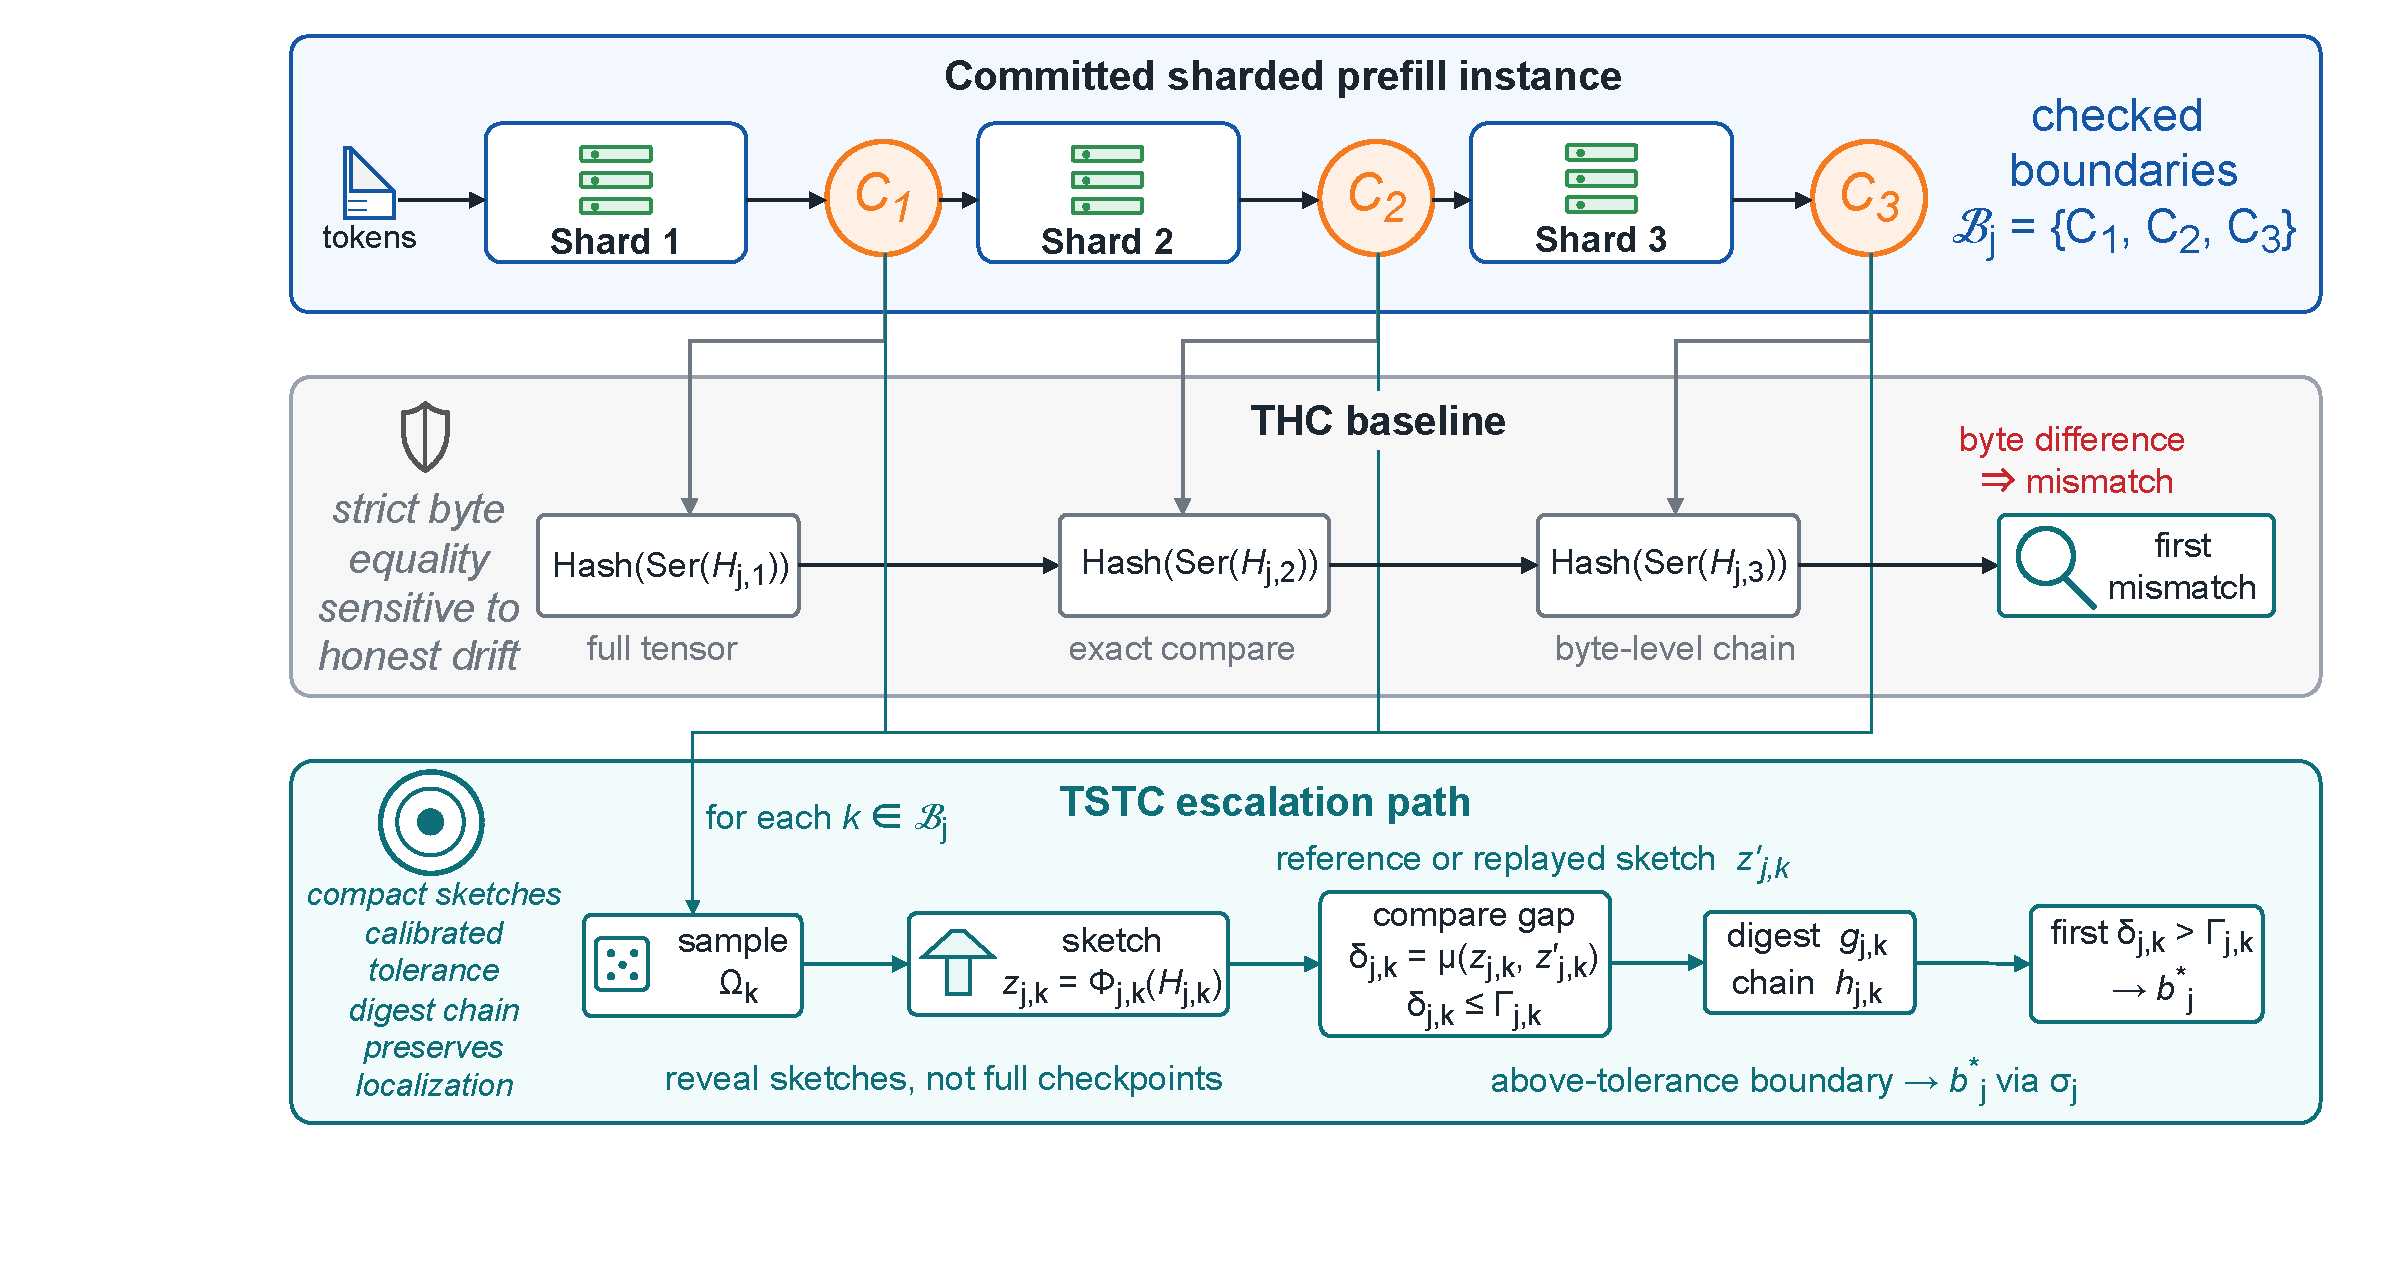
\includegraphics[width=0.98\linewidth]{fig_tstc_mechanism.drawio.pdf}
	\caption{\textbf{TSTC dispute escalation.}
		THC hashes full checkpoints strictly at checked shard boundaries.
		TSTC instead treats each boundary as a compact checkpoint sketch,
		compares challenged and reference sketches under calibrated tolerance,
		and chains boundary evidence to preserve first-mismatch
		localization under heterogeneous execution. Scalar-coordinate and
		projected-token sketches share this challenge protocol; only the
		sketch statistic changes.}
	\Description{A verification mechanism diagram showing three
		shard-boundary checkpoints on the prefill path. The strict tensor-hash
		baseline hashes full checkpoints, while TSTC uses compact checkpoint
		sketches, calibrated tolerance, digest binding, and first-mismatch
		localization for challenge-time arbitration.}
	\label{fig:tstc}
\end{figure}

\paragraph{Routine screening.}
The first layer decides whether a result can settle cheaply. Direct requester
acceptance, lightweight semantic filters, or stronger judge models can flag
suspicious outputs~\cite{zheng2023judging,liu2025polylink}, but they do not
identify the responsible shard boundary.

\paragraph{Checkpoint-sketch evidence.}
When a task is challenged, the verifier consumes checkpoint-sketch evidence
\(E_j\) derived from the shard-boundary states of the committed execution
plan. Let \(\mathcal{B}_j\) be the checked boundary set in
\(\vartheta_j\). For boundary \(k\), let
\(H^{\mathsf{prov}}_{j,k}\) denote the challenged provider-side checkpoint
state and \(H^{\mathsf{ref}}_{j,k}\) denote the reference or replayed
checkpoint state under the committed context. The verification policy specifies
a sketch function \(\Phi_{j,k}\), a comparison rule \(\mu_{j,k}\), a
tolerance \(\Gamma_{j,k}\), and a seed-derivation context for each checked
boundary. The provider-side evidence for boundary \(k\) is a compact sketch
\(z_{j,k}=\Phi_{j,k}(H^{\mathsf{prov}}_{j,k})\), rather than the full
checkpoint tensor.

A strict tensor hash chain (THC), shown as the baseline in
Figure~\ref{fig:tstc}, is the degenerate case in which the
``sketch'' is the full serialized checkpoint tensor and comparison is exact
equality. It localizes mismatches, but any honest byte-level drift becomes a
mismatch.

\paragraph{Tolerance-aware sketch tensor chain.}
TSTC generalizes THC by replacing full-tensor equality with compact sketch
comparison under calibrated tolerance. For each checked boundary, providers
commit to or make retrievable a sketch digest before challenge resolution. A
simple chain form is
\begin{equation}
g_{j,k}=\mathsf{Hash}(\mathsf{Ser}(z_{j,k})\,\|\,k\,\|\,\mathsf{ctx}_j),
\;
h_{j,k}=\mathsf{Hash}(h_{j,k-1}\,\|\,g_{j,k}),
\label{eq:tstc-chain}
\end{equation}
with \(h_{j,0}=\epsilon\), where \(\|\) denotes byte-string concatenation and
\(\mathsf{Ser}(\cdot)\) denotes canonical tensor serialization. The chain binds
the order and identity of checkpoint evidence; the challenged reveal of
\(z_{j,k}\) lets the verifier compare against a reference or replayed sketch.

The committed policy fixes this timing. Placement commits
\((\mathcal{G}_j,\sigma_j,\vartheta_j)\), including checked boundaries, sketch
mode, tolerances, seed context, and replay/reference path. Execution makes each
boundary digest retrievable before challenge resolution; a challenge opens only
requested sketches, which must match their digests. The verifier derives the
reference sketch under the committed context, and missing, malformed, or
digest-invalid evidence is treated as a settlement-visible protocol violation
rather than benign drift.

On challenge, the provider opens the sketch \(z_{j,k}\) for boundary \(k\).
The verifier recomputes the opened digest \(\hat{g}_{j,k}\) using the hash in
Equation~\ref{eq:tstc-chain} and checks that it matches the digest \(g_{j,k}\)
bound by the committed chain \(h_{j,k}\). If this check passes, the verifier
derives the reference sketch
\(z'_{j,k}=\Phi_{j,k}(H^{\mathsf{ref}}_{j,k})\) and computes
\(\delta_{j,k}=\mu_{j,k}(z_{j,k},z'_{j,k})\). If
\(\delta_{j,k}\le\Gamma_{j,k}\), boundary \(k\) is accepted; otherwise the first
over-tolerance boundary is \(b^\star_j\).

\paragraph{Sketch instantiations.}
TSTC is therefore a checkpoint-sketch family rather than one equality test.
For a sketch policy \(\theta\), the provider-side evidence is generated as
\(z_{j,k}=\Phi_{\theta}(H^{\mathsf{prov}}_{j,k})\). The verifier's
challenge-time computation is
\begin{equation}
z'_{j,k}=\Phi_{\theta}(H^{\mathsf{ref}}_{j,k}),\;\;\;
\delta_{j,k}=\mu_{\theta}(z_{j,k},z'_{j,k}),\;\;\;
\delta_{j,k}\le\Gamma_{j,k}.
\end{equation}
Here \(\Phi_{\theta}\) is the sketch function and \(\mu_{\theta}\) is the
comparison rule under sketch policy \(\theta\).

The scalar-coordinate instance treats checkpoint sketching as a sparse
token-channel projection:
\begin{equation}
\Phi_{\mathrm{scalar}}(H_{j,k})
  = P_{\Omega_{j,k}}\mathrm{vec}(H_{j,k}),
\end{equation}
where \(P_{\Omega_{j,k}}\) selects a small set of coordinates from the
checkpoint tensor \(H_{j,k}\). Its comparison rule is the largest selected-coordinate
absolute gap,
\begin{equation}
\mu_{\mathrm{scalar}}(z_{j,k},z'_{j,k})
  = \|z_{j,k}-z'_{j,k}\|_{\infty}
  = \max_{1\le r\le|\Omega_{j,k}|}|z_{j,k,r}-z'_{j,k,r}|.
\end{equation}
The boundary is accepted when this gap is within the calibrated tolerance in
\(\Gamma_{j,k}\).

The projected-token instance treats
\(H_{j,k}\in\mathbb{R}^{T\times D}\) as a token-level representation matrix.
It derives a seeded projection \(R_{j,k}\in\mathbb{R}^{D\times d}\). The
sketch is still denoted \(z_{j,k}\), but in this instance it is a
token-sketch matrix:
\begin{equation}
\Phi_{\mathrm{proj}}(H_{j,k})
  =\mathrm{NormalizeRows}(H_{j,k}R_{j,k})\in\mathbb{R}^{T\times d}.
\end{equation}
For provider and reference sketches \(z_{j,k}\) and \(z'_{j,k}\),
\(z_{j,k,t}\) denotes the row for token \(t\). The comparison rule is a
token-wise projected cosine gap:
\begin{equation}
\mu_{\mathrm{proj}}(z_{j,k},z'_{j,k})
  = \frac{1}{T}\sum_{t=1}^{T}
    \left(1-\cos(z_{j,k,t},z'_{j,k,t})\right).
\end{equation}
Across these instances, the challenge protocol, digest binding, calibrated
tolerance, and first-mismatch localization are unchanged; only the
checkpoint-sketch statistic changes.

\paragraph{Calibration.}
The tolerance map \(\Gamma_j\) is calibrated from honest heterogeneous runs
for the relevant model, boundary, device and backend mix, and sketch policy.
\system does not assume one universal mode: global tolerances can be robust,
while boundary-specific tolerances help when checkpoints have different drift
scales. Calibration also tells placement which pairs are stable, need richer
sketches, or remain poor candidates for cheap adjudication.

\paragraph{Challenge semantics.}
\label{subsec:semantics}
The verifier consumes \(E_j\) under \(\pi_j\) and \(\vartheta_j\), and
returns a status and localization pair \((s_j,b^\star_j)\). Here
\(s_j\in\{\mathsf{accept},\mathsf{mismatch}\}\). If no checked boundary
exceeds its tolerance, the challenge returns
\((\mathsf{accept},\bot)\). Otherwise \(b^\star_j\) is the first checked
boundary whose sketch comparison exceeds tolerance, interpreted through
\(\sigma_j\). TSTC is not a cryptographic proof of semantic correctness; it is
a bounded arbitration primitive that reduces false disputes while preserving
localized evidence for material divergence. Attacks outside the challenged
evidence and fully colluding self-consistent groups remain outside this
guarantee, and these limits are visible to placement.

\subsection{Settlement and Feedback}
\label{subsec:settlement-feedback}

Challenge results feed into contract-mediated settlement. If no challenge is
raised, or if verification returns \(\mathsf{accept}\), providers in
\(\mathcal{G}_j\) are paid according to the task policy. If verification
returns \(\mathsf{mismatch}\) with boundary \(b^\star_j\), the system maps
that boundary through \(\sigma_j\) and associates the failure with the relevant
provider or adjacent shard pair.

The settlement state machine supports normal settlement, provider penalties,
challenge forfeiture, and verifier-side penalties for protocol violations. The
systems requirement is that settlement derive from the same committed placement
and verification policy used for disclosure and challenge interpretation.
Completed tasks, failed challenges, confirmed fraud, unresolved disputes, and
observed drift update future placement signals.





%------------------------------------------------------------
\section{Prototype Implementation}
\label{sec:implementation}
%------------------------------------------------------------

\paragraph{Prototype scope.}
\system is implemented as a runtime-agnostic prototype for the interfaces
used in the evaluation: public task publication, placement commitment,
selective delivery, controlled shard execution, checkpoint-sketch
verification, and settlement feedback. The coordination component maintains
task, provider, placement, challenge, and settlement records, but only compact
commitments and outcomes are durable. Ciphertexts, access packages, shard
execution, and sketch objects remain off chain. The prototype is therefore
not a production scheduler or strategy-proof market; it validates that the
placement, delivery, execution, verification, and settlement hooks can be tied
to one committed accountability record.

\paragraph{Selective delivery path.}
The delivery component follows Section~\ref{subsec:selective-delivery}. The
requester encrypts the payload
once, publishes the ciphertext to IPFS as a content-addressed object, and
sends encrypted access packages only to providers in the committed
group. The orchestrator sees the placement record but is not on the access
tuple disclosure path. The delivery evaluation compares this
privacy-preserving delivery (PPD) path against replicated payload delivery
(RPD), which sends a full encrypted payload independently to each selected
provider.

\paragraph{Verifier harness.}
For verification and placement risk measurement, we use a controlled PyTorch
sharded inference harness rather than binding \system to one collaborative
runtime. The harness partitions modules according to \(\sigma_j\), transfers
or captures shard-boundary activations, and focuses on three prefill
checkpoints \(C_1\), \(C_2\), and \(C_3\). It can retain full tensors for instrumentation, but
the settlement-facing evidence is a digest, compact sketch, or challenged
sketch reveal. A common checkpoint-sketch interface implements THC,
scalar-coordinate TSTC, and projected-token TSTC; calibration profiles are
learned from honest runs disjoint from evaluation prompts and versioned by
model, checkpoint set, device/backend mix, sketch mode, and tolerance rule.
The same harness injects controlled checkpoint perturbations for sensitivity
studies and reports detection and first-mismatch localization.


\paragraph{Artifact.}
The anonymized artifact at
\url{https://anonymous.4open.science/r/veriedge-artifact-E961/} provides an
interface-level prototype and auxiliary reproducibility material. It includes
verifier-profile tables, replay/delivery scripts, plotting code, Wilson 95\%
intervals for verifier-profile FPR/TPR from held-out counts, and a small
runnable demo that connects placement admission, selective delivery, TSTC
challenge localization, and a mock ledger/settlement interface. It is not a
production deployment.




\section{Evaluation}
\label{sec:evaluation}

Our evaluation tests the paper's central claim: low-cost verifiability is a
placement-visible property of a device/backend execution mix, a checkpoint
sketch, and a verifier budget. We organize the evidence in placement-first
order:
\begin{itemize}[leftmargin=1.5em]
	\item \textbf{Q1:} How does a measured verification profile change
	placement admission and policy replay?
	\item \textbf{Q2:} Does committed placement also reduce requester-side
	delivery work by defining who receives task access?
	\item \textbf{Q3:} Which heterogeneous stack pairs become low-risk,
	high-risk, or inadjudicable under compact checkpoint sketches?
	\item \textbf{Q4:} Which sketch statistics, budgets, and tamper families
	explain the resulting verifier profiles?
	\item \textbf{Q5:} What payload and challenge-time cost do stronger
	checkpoint sketches add?
\end{itemize}

\subsection{Methodology and Scope}
\label{subsec:eval-methodology}

Our evaluation uses one common accountability unit: a committed execution
group, shard map, and verifier mode before task disclosure. We evaluate this
unit with a coordination prototype, replayed placement policies, delivery-path
microbenchmarks, and a controlled PyTorch-based sharded-inference driver. The
verification driver runs sharded prefill inference and captures checkpoint
states at shard boundaries. Each trace exposes three prefill shard-boundary
checkpoints, and each verifier compares a candidate checkpoint sketch against
a reference sketch under a calibrated tolerance.

Unless otherwise noted, verifier tolerances are calibrated only from honest
heterogeneous calibration prompts and then evaluated on disjoint held-out
prompts. Scalar sketches estimate coordinate-gap tolerances; projected-token
sketches estimate projected-cosine gap thresholds. Placement replay consumes
the measured verifier profiles produced by these calibration and evaluation
runs, while delivery measurements use the same placement-defined access
boundary: only selected providers receive decryptable access material.
Placement replay uses the measured verifier profiles as fixed
inputs to compare policy decisions under controlled workloads.

Table~\ref{tab:eval-execution-stacks} defines the stack labels used in the
experiments. Each row is a three-stage prefill path: C1 covers layers 0--7, C2
covers layers 8--15, and C3 covers layers 16--23. The stacks use two Mac mini
M4 devices through Apple MPS and one RTX3090 Linux server through CUDA. FP16,
BF16, and FP32 denote half-, bfloat16-, and single-precision execution;
Metal-int8 denotes the Apple Metal 8-bit quantization path. When two labels are
later written as A/B, the same prompts are replayed under the two paths and the
same shard-boundary checkpoint sketches are compared.
These labels are experimental identifiers, not algorithm variables.

\begin{table}[t]
\centering
\caption{Hardware/backend paths used for paired checkpoint captures.}
\label{tab:eval-execution-stacks}
\scriptsize
\setlength{\tabcolsep}{2pt}
\newcommand{\stacksep}{\noalign{\vskip 1.2pt{\color{black!18}\hrule height 0.25pt}\vskip 1.2pt}}
\begin{tabular}{@{}c@{\hspace{1.25em}}l@{\hspace{0.35em}}>{\raggedright\arraybackslash}p{0.43\linewidth}@{\hspace{0.45em}}l@{}}
\toprule
\textbf{Stack} & \multicolumn{2}{l}{\textbf{Three-stage path}} & \textbf{Execution mix} \\
\midrule
\multirow{3}{*}{A}
  & \textbf{C1:} & Apple M4/MPS FP16+Metal-int8
  & \multirow{3}{*}{\shortstack[l]{mixed vendor;\\C1 quantized}} \\
  & \textbf{C2:} & Apple M4/MPS BF16 & \\
  & \textbf{C3:} & RTX3090/CUDA FP32 & \\
\stacksep
\multirow{3}{*}{B}
  & \textbf{C1:} & Apple M4/MPS BF16
  & \multirow{3}{*}{\shortstack[l]{Apple BF16 prefix;\\RTX final}} \\
  & \textbf{C2:} & Apple M4/MPS BF16 & \\
  & \textbf{C3:} & RTX3090/CUDA FP32 & \\
\stacksep
\multirow{3}{*}{C}
  & \textbf{C1:} & RTX3090/CUDA BF16
  & \multirow{3}{*}{\shortstack[l]{cross-vendor;\\BF16/FP32}} \\
  & \textbf{C2:} & Apple M4/MPS BF16 & \\
  & \textbf{C3:} & RTX3090/CUDA FP32 & \\
\stacksep
\multirow{3}{*}{D}
  & \textbf{C1:} & RTX3090/CUDA FP32
  & \multirow{3}{*}{\shortstack[l]{RTX-heavy;\\FP32/BF16}} \\
  & \textbf{C2:} & Apple M4/MPS BF16 & \\
  & \textbf{C3:} & RTX3090/CUDA FP32 & \\
\stacksep
\multirow{3}{*}{E}
  & \textbf{C1:} & RTX3090/CUDA FP32
  & \multirow{3}{*}{\shortstack[l]{FP32;\\mixed backend}} \\
  & \textbf{C2:} & Apple M4/MPS FP32 & \\
  & \textbf{C3:} & Apple M4/MPS FP32 & \\
\stacksep
\multirow{3}{*}{F}
  & \textbf{C1:} & Apple M4/MPS FP32
  & \multirow{3}{*}{\shortstack[l]{Apple-only\\FP32 control}} \\
  & \textbf{C2:} & Apple M4/MPS FP32 & \\
  & \textbf{C3:} & Apple M4/MPS FP32 & \\
\bottomrule
\end{tabular}
\end{table}

We report honest-heterogeneous false-positive rate (FPR), tamper true-positive
rate (TPR), first-mismatch localization accuracy (LocAcc), sketch payload, and
challenge latency. We use the following shorthand: ``scalar\(N\)'' denotes
scalar-coordinate TSTC with \(N\) sparse token-channel samples per checkpoint
(scalar16 reveals \(16\) floats, or \(64\) bytes); ``projcos\(d\)'' denotes
projected-token TSTC that projects each checked token hidden state to dimension
\(d\) and compares token-wise cosine gaps (with \(T=16\), projcos4 reveals
\(T d=64\) floats, or \(256\) bytes); ``projscalar1\_abs'' denotes a
one-dimensional projected-token sketch that compares calibrated absolute gaps,
so it remains sensitive to vector norm. Strict tensor hashing (THC) is the
brittle bit-exact baseline: in real heterogeneous captures it rejects honest
runs whenever byte-level checkpoint serialization differs.

\subsection{Closed-Loop Verifiability-Constrained Placement}
\label{subsec:eval-placement}

We replay placement policies over a fixed workload, candidate set, and measured
verifier profiles to test whether verifiability changes admission before task
disclosure. This controlled decision replay fixes the workload, candidates, and
profile keys so differences reflect admission, queue-aware scoring, and
verifier-mode selection. The matrix contains 34 rows keyed by stack pair and
sketch mode over C1--C3; for example, A/B+\allowbreak{}projcos4 records the
Table~\ref{tab:eval-execution-stacks} paths A and B under the projcos4 sketch.
For the main \(\alpha=0.10,\beta=0.90\) target, 19 rows satisfy held-out FPR
\(\le\alpha\), primary material-tamper TPR \(\ge\beta\),
\(S^{\max}=3072\) bytes per trace, and \(C^{\max}=5.0\) ms verifier latency;
the rest are infeasible. Hard filtering rejects such candidates, while
adaptive verifier-mode selection tries to keep them feasible by choosing a
stronger sketch. False-dispute risk is the task challenge probability times
the selected profile's held-out honest FPR. The supplementary material reports
the full matrix, replay configuration, policy semantics, and exact queued-8
metrics.

We compare three policy classes. Latency-oriented policies rank candidates by
network cost, queue cost, or both, but do not reject verifier-infeasible keys.
Verifiability-constrained policies first apply the hard admission test in
Equation~\ref{eq:placement-feasibility} and then rank only admitted candidates.
Adaptive-verifier policies keep the candidate group when possible, but upgrade
to the cheapest sketch satisfying the task's
\((\alpha,\beta,S^{\max},C^{\max})\) targets; if none exists, the candidate is
rejected.

\begin{figure*}[t]
	\centering
	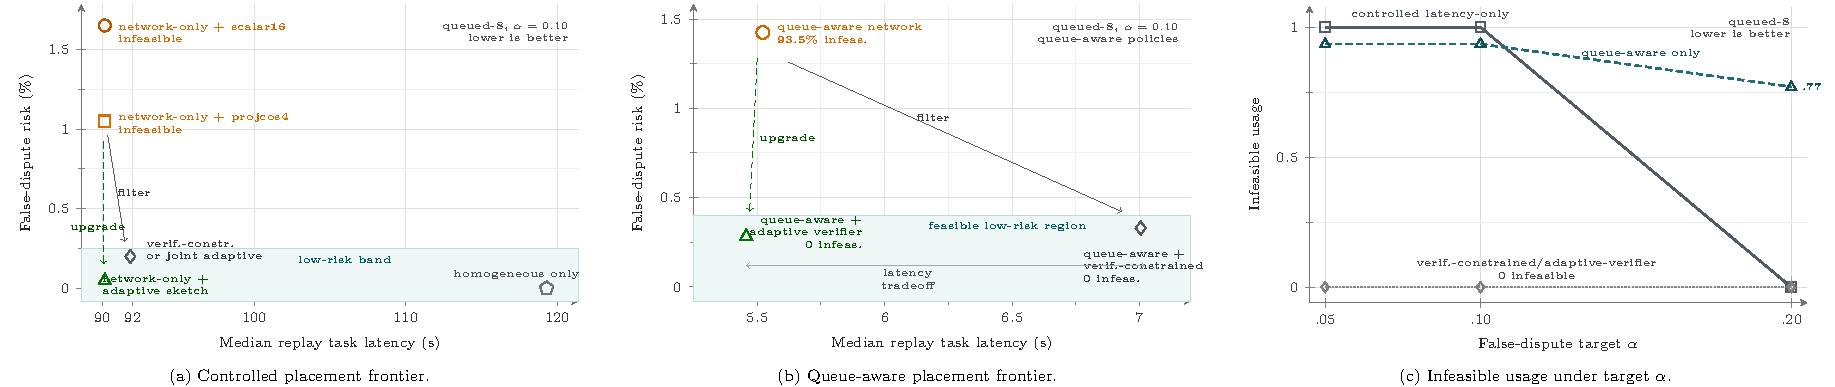
\includegraphics[width=\textwidth]{fig_exp_tikz/fig_placement_replay_1x3.pdf}
	\caption{Closed-loop placement replay using measured verifier profiles. The
		controlled replay isolates the admission mechanism, while the queue-aware
		replay adds current waiting time to the placement score. Network- and
		queue-aware latency policies can still select infeasible verifier-profile keys;
		verifiability-constrained and adaptive-verifier policies filter or upgrade
		those choices before task disclosure.}
	\Description{Three panels showing placement frontiers and alpha sensitivity for
		the closed-loop placement replay.}
	\label{fig:placement-replay-panels}
\end{figure*}

We replay the 200 evaluation prompts under two arrival patterns: a
low-pressure single pattern and a queued-8 burst pattern. The main placement
readout in Figure~\ref{fig:placement-replay-panels} uses queued-8, where eight
tasks arrive together and a new burst arrives every 0.25 s. Panel (a)
evaluates non-queue-aware policies on this same bursty workload to isolate
verifier admission; panel (b) adds current candidate queue wait to the placement
score; and panel (c) sweeps the false-dispute target \(\alpha\). Median replay
task latency is modeled service time plus queue wait when queues are enabled;
verifier challenge time is reported separately.



Panel (a) shows the value of hard admission. With the same fixed projcos4
sketch, network-aware placement selects infeasible verifier-profile keys for all
admitted queued-8 tasks. Verifiability-constrained placement checks the measured profile before
disclosure and reduces infeasible usage from \(1.000\) to \(0.000\), while
reducing false-dispute risk from \(0.0105\) to \(0.0020\). Replay goodput changes
only modestly, from \(1.079\) to \(1.060\), because the policy avoids a
low-latency but inadmissible group. A network-aware adaptive policy also reaches
zero infeasible usage while preserving the latency baseline's replay goodput by
upgrading the selected group to a feasible verifier mode.

The queue-aware replay in Figure~\ref{fig:placement-replay-panels}(b) separates
load balancing from verifiability. Queue-aware network placement reaches
goodput \(12.266\) with median task latency \(5.522\) s, but still selects
infeasible profile keys in \(93.5\%\) of admitted tasks. Hard constraints
remove those choices at higher latency, while queue-aware adaptive verifier
selection reaches zero infeasible usage with nearly the same goodput
(\(12.251\) versus \(12.266\)). The \(\alpha\) sweep in
Figure~\ref{fig:placement-replay-panels}(c) confirms that this is not a
single-threshold artifact: for \(\alpha\in\{0.05,0.10,0.20\}\), constrained
and adaptive policies keep infeasible usage at \(0.000\), whereas the
queue-aware network policy remains infeasible on \(0.935,0.935,\) and \(0.770\)
of admitted tasks. Thus measured verifier behavior is useful before execution:
it turns heterogeneous verifiability into a placement-time admission and
verifier-selection constraint rather than an after-the-fact checker.

\subsection{Selective Delivery Microbenchmark}
\label{subsec:eval-delivery}

Placement also defines the data boundary: only selected providers receive
decryptable task-access material. We evaluate this mechanism with a calibrated
delivery-path group-size microbenchmark rather than a live multi-provider
deployment. The experiment uses a 100MB encrypted payload,
\(k\in\{1,2,4,8\}\) selected providers, and 30 runs per cell. It combines
measured local cryptographic costs with explicit LAN/WAN bandwidth and RTT
profiles to compare requester-side disclosure cost as placement width grows.
A separate live local-store
supplement verifies the protocol hygiene requirements: each run creates a
fresh ciphertext object, derives a content-hash object key, and has providers
fetch and hash-check the stored ciphertext. We use that supplement to rule out
cache reuse, not as the source of the LAN/WAN latency claim.

We isolate the committed-disclosure mechanism with a 100MB payload and compare
privacy-preserving delivery (PPD) against replicated payload delivery (RPD).
Both paths transfer encrypted data; the difference is where replication
occurs. RPD sends a full encrypted payload to each selected provider, while
PPD publishes one ciphertext object and releases small locator-and-key
packages after the placement commitment.

\begin{table}[t]
\centering
\caption{Selective-delivery microbenchmark for a 100MB encrypted payload. Reductions compare PPD against RPD; requester-egress reduction is independent of the LAN/WAN profile.}
\label{tab:delivery-sweep}
\scriptsize
\setlength{\tabcolsep}{4.5pt}
\begin{tabular}{rrrr}
\toprule
\textbf{\(k\)} & \textbf{LAN med. red.} & \textbf{WAN med. red.} & \textbf{Req. egress red.} \\
\midrule
1 & \(-99.1\%\) & \(-50.6\%\) & \(0.0\%\) \\
2 & \(-0.3\%\) & \(24.5\%\) & \(50.0\%\) \\
4 & \(49.7\%\) & \(62.2\%\) & \(75.0\%\) \\
8 & \(74.8\%\) & \(81.1\%\) & \(87.5\%\) \\
\bottomrule
\end{tabular}
\end{table}

Table~\ref{tab:delivery-sweep} shows that PPD becomes increasingly beneficial
as the selected group grows. It is not universally faster:
at \(k=1\), PPD is slower because the publication and access-package path adds
coordination overhead without any requester-side replication to eliminate; its
benefit appears with group width because it avoids RPD's \(O(kS)\) requester
egress. At \(k=8\), median all-providers-ready latency
falls from \(6.82\) s to \(1.72\) s on LAN and from \(160.10\) s to
\(30.27\) s on WAN, while requester egress falls from \(800\) MB to about
\(100\) MB. The result supports the placement-boundary claim: once the group
is fixed, the requester can avoid repeated payload-sized transfers while still
releasing decryptable access only to selected providers.

\subsection{Verifier Profiles on Heterogeneous Pairs}
\label{subsec:eval-pair-family}

Table~\ref{tab:pair-family-projcos} compares scalar-coordinate TSTC against
projected-token TSTC on four heterogeneous stack pairs. For each stack pair,
we use 40 calibration prompts and 200 held-out evaluation prompts. Each cell
reports held-out FPR/TPR after selecting the tolerance from calibration
prompts. We report point estimates in the main table for space; the artifact
includes Wilson 95\% intervals for the corresponding FPR/TPR estimates from
held-out counts. Tolerances are selected on calibration prompts and evaluated on
disjoint held-out prompts.
Across these runs, both scalar-coordinate and projected-token sketches detect
the injected tamper cases: every listed TPR is \(1.000\). The separation is in
honest-heterogeneous FPR. Scalar16 still produces FPR between \(0.090\) and
\(0.245\), because a sparse scalar sketch observes individual token-channel
values where benign backend and precision drift can overlap the deviations
caused by tampering. Projected-token sketches move the comparison to
token-level representation direction, which preserves more checkpoint geometry
and reduces sensitivity to isolated coordinate drift.

\begin{table}[t]
\centering
\caption{Held-out FPR/TPR on heterogeneous stack-pair captures. Each operating point is selected on calibration prompts and evaluated on held-out prompts.}
\label{tab:pair-family-projcos}
\scriptsize
\setlength{\tabcolsep}{3pt}
\begin{tabular}{lccccc}
\toprule
\textbf{Stack pair} & \textbf{Scalar risk} & \textbf{Scalar16} & \textbf{ProjCos4} & \textbf{ProjCos8} & \textbf{ProjCos16} \\
\midrule
A/B & medium & .150 / 1.000 & .020 / 1.000 & .080 / 1.000 & .120 / 1.000 \\
A/C & medium & .110 / 1.000 & .045 / 1.000 & .075 / 1.000 & .135 / 1.000 \\
A/D & low & .090 / 1.000 & .020 / 1.000 & .065 / 1.000 & .065 / 1.000 \\
B/D & hard & .245 / 1.000 & .075 / 1.000 & .075 / 1.000 & .065 / 1.000 \\
\bottomrule
\end{tabular}
\end{table}

We classify the scalar baseline risk from held-out scalar16 FPR: low for
\(<0.10\), medium for \(0.10\)--\(0.20\), and hard for \(>0.20\). More
generally, a hard stack pair is one where, after calibration, the chosen sketch
and budget cannot keep honest FPR below the target \(\alpha\) and tamper TPR
above \(\beta\). Hardness is therefore relative to the sketch statistic,
budget, and target profile; it is not a permanent label for a device alone.
Projected-token TSTC improves the operating window across the evaluated stack
pairs. On B/D, the scalar16 sketch has FPR/TPR \(=0.245/1.000\); projcos4
lowers FPR to \(0.075\), and projcos16 lowers it further to \(0.065\), while
preserving TPR and LocAcc at \(1.000\). Easier pairs can favor the most
compressed projected sketch, but the hardest pair benefits from a slightly
larger projection dimension; the verifier should therefore choose the sketch
dimension from calibration rather than assume that the smallest sketch is
always the best operating point. The result is not a claim that all
heterogeneous stack pairs are solved, but it shows that retaining token-level
representation geometry can turn a high-risk stack pair into a lower-risk
placement candidate.

\subsection{Sketch Statistic Versus Budget}
\label{subsec:eval-equal-budget}

A natural question is whether projected-token TSTC performs better simply
because it reveals more numbers. Table~\ref{tab:equal-budget-sketches}
compares equal-budget operating points on the A/B stack-pair setting. The key
separation is that
scalar64 and projcos4 both reveal \(256\) bytes per checkpoint, but scalar64
has held-out FPR \(0.415\), while projcos4 has FPR \(0.020\), with both at TPR
and LocAcc \(1.000\). Thus the benefit is not payload size alone; the
statistic matters.

\begin{table}[t]
	\centering
	\caption{Equal-budget sketch comparison on A/B stack-pair captures.}
	\label{tab:equal-budget-sketches}
	\scriptsize
	\setlength{\tabcolsep}{4.5pt}
	\begin{tabular}{@{}lccccc@{}}
		\toprule
		\textbf{Metric} &
		\textbf{scalar16} &
		\textbf{scalar64} &
		\textbf{projscalar1\_abs} &
		\textbf{projcos4} &
		\textbf{projcos16} \\
		\midrule
		B/ckpt & 64 & 256 & 64 & 256 & 1024 \\
		FPR & .150 & .415 & .000 & .020 & .120 \\
		TPR & 1.000 & 1.000 & 1.000 & 1.000 & 1.000 \\
		LocAcc & 1.000 & 1.000 & 1.000 & 1.000 & 1.000 \\
		\bottomrule
	\end{tabular}
\end{table}



The projected-scalar bridge is included to separate two explanations for the
projected-token result: payload size and the statistic being measured. It keeps
one random-projection scalar per token and compares absolute gaps, so it is
norm-sensitive rather than cosine-only. At \(64\) bytes per checkpoint,
projscalar1\_abs achieves FPR \(0.000\) and TPR \(1.000\) in the A/B
comparison. To check that this zero-FPR point is not tied to a
lucky sketch seed, we repeat the projected-scalar comparison with five
independent sketch seeds across A/B, A/B-RTXint8, A/C, A/D, B/D, and E/F.
Among these pairs, E/F is a same-precision FP32 backend-control pair: E keeps
FP32 precision but crosses CUDA/MPS backends, while F stays on Apple/MPS FP32.
The resulting projscalar1\_abs profile has mean held-out FPR \(0.0073\), max
FPR \(0.025\), and minimum primary-material TPR \(1.000\). We treat this as a
diagnostic and hybrid-verifier component, not as a replacement for
projected-token TSTC: a one-dimensional projection has an explicit null space,
and Section~\ref{subsec:eval-material-tamper} shows that a projection-aware
null-space attack can evade it.

\subsection{Material-Tamper Coverage and Blind Spots}
\label{subsec:eval-material-tamper}

The tamper study separates statistical perturbations (Gaussian noise) from
material attacks (stale substitution, wrong-shard output, layer skip, and
scale perturbation) that better resemble faulty or dishonest execution.
Figure~\ref{fig:material-tamper-focus} visualizes the main pattern; the
supplementary material reports the exact A/B and B/D attack-family TPRs.
Projected-token TSTC is strong on direction-changing attacks: stale
substitution, wrong-shard output, and layer skip all reach TPR \(1.000\) for
projcos4 on the shown stack pairs. Its limitation is equally clear:
direction-preserving scale perturbations are almost invisible to a cosine-only
sketch because row normalization removes most norm information.

\begin{figure}[!t]
\centering
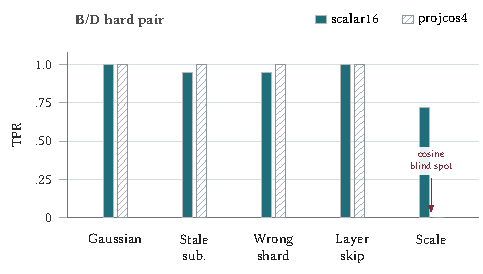
\includegraphics[width=0.98\linewidth]{fig_exp_tikz/fig_material_tamper_focus.pdf}
\caption{Material tamper focus on the B/D hard pair. The plot shows that projcos4 detects direction-changing attacks but misses direction-preserving scale perturbations.}
\Description{A panel comparing true-positive rates across material tamper families for scalar-coordinate and projected-token sketches.}
\label{fig:material-tamper-focus}
\end{figure}

The output-affecting subset confirms the same boundary at next-token top-\(k\)
level. For projcos4, output-affecting TPR is \(1.000\) for Gaussian,
cross-prompt stale substitution, wrong-shard output, and layer skip, but only
\(0.0107\) for scale perturbation. Scalar16 is less reliable on semantic
substitution and layer skip, with output-affecting TPR around \(0.75\), but it
retains some sensitivity to scale perturbation because it compares absolute
coordinate gaps. On A/B, the output-affecting Gaussian and
layer-skip attacks substantially change the next-token neighborhood
(mean top-5 Jaccard \(0.002\) and \(0.174\)), while scale perturbation is
much closer to the original output distribution (mean top-5 Jaccard \(0.898\))
and remains the cosine blind spot. The projscalar1\_abs extension complements both: it detects
ordinary Gaussian, stale, wrong-shard, layer-skip, and scale perturbations at
TPR \(1.000\), but a projection-aware null-space attack has TPR \(0.000\).
This is the right scientific boundary: norm-sensitive projections are useful
hybrid components, but no single low-cost statistic should be claimed as an
adaptive security proof.

\subsection{Verifier Payload and Challenge Runtime}
\label{subsec:eval-overhead}

Stronger sketches are not free. Table~\ref{tab:verifier-overhead} reports
payload and challenge latency for the equal-budget setting. Projcos4 sends
\(256\) bytes per checkpoint and \(768\) bytes for a three-checkpoint trace;
projcos16 sends \(3072\) bytes per trace. Challenge-time latency remains in
the few-millisecond range for all variants, increasing from roughly \(3.6\) ms
for scalar16 to roughly \(3.8\) ms for projcos4 and \(4.0\) ms for projcos16.

\begin{table}[!t]
\centering
\caption{Checkpoint-sketch payload and challenge-time verifier latency.}
\label{tab:verifier-overhead}
\scriptsize
\setlength{\tabcolsep}{3pt}
\begin{tabular}{lrrrr}
\toprule
\textbf{Variant} & \textbf{B/ckpt} & \textbf{B/trace} & \textbf{Honest ms} & \textbf{Tamper ms} \\
\midrule
scalar16 & 64 & 192 & 3.603 & 3.382 \\
scalar64 & 256 & 768 & 3.469 & 3.403 \\
projscalar1\_abs & 64 & 192 & 3.709 & 3.814 \\
projcos4 & 256 & 768 & 3.798 & 3.684 \\
projcos16 & 1024 & 3072 & 4.041 & 3.943 \\
\bottomrule
\end{tabular}
\end{table}

These numbers support the intended cost claim: projected-token TSTC increases
reveal payload, but remains compact enough for challenge-time verification or
for placements classified as high-risk under cheaper sketches. We do not
claim it is nearly free; the orchestrator should account for the sketch budget
when selecting a placement and challenge policy.

\subsection{Evaluation Takeaways}
\label{subsec:eval-takeaways}

The experiments support three conclusions. Measured verifier profiles change
placement before disclosure by removing or upgrading inadmissible candidates;
committed placement also acts as the data boundary for selective access; and
the profile itself is sketch-dependent, with scalar, projected-token, and
norm-sensitive sketches exposing different cost--risk operating points. These
are scoped systems results, not universal correctness guarantees.


\section{Discussion}
\label{sec:discussion}
\paragraph{Profile lifecycle.}
\system treats verifier measurements as placement inputs, which creates a
profile lifecycle rather than a one-time benchmark. A profile is calibrated
for a model, boundary set, device/backend path, sketch mode, and tolerance
rule; used for admission before disclosure; updated after challenges; and
expired when software, kernels, model versions, or hardware change. Missing or
stale profiles are therefore handled conservatively: the candidate is rejected,
assigned a stronger sketch, or routed through calibration depending on policy.
Calibration is not free, but unlike per-task proof generation it can be
amortized across many tasks until drift invalidates the profile. Coarse
profiles reduce measurement cost but may hide a risky boundary; our current
aggregation uses conservative max/min rules so one risky boundary cannot be
washed out by averages. The ledger need only commit decisions and settlement
outcomes, while calibration, inference, profile maintenance, and sketch
comparison remain off the latency-critical chain path.

\paragraph{Scope and fallback.}
TSTC profiles should not be read as adaptive cryptographic guarantees. They
are calibrated arbitration evidence under an explicit sketch budget and threat
model, and the projected-scalar null-space result shows that a statistic that
works well against ordinary perturbations can still have a white-box blind
spot. A practical deployment should treat verifier modes as an ordered menu:
low-risk tasks can use small sketches, risky or stale profiles can be upgraded
to richer sketches or replay, and high-assurance tasks may require heavier
proof or trusted-execution mechanisms outside the routine path. Our study is
also scoped to prefill shard-boundary checkpoints, one model family, a small
set of Apple/MPS and NVIDIA/CUDA paths, controlled material tamper, and a
fixed replay generator rather than a production scheduler. Thus \system
exposes verifiability as a measurable placement constraint, but continued
profiling is still needed as models, devices, and verifier budgets change.

\section{Related Work}
\paragraph{Collaborative LLM inference}
Edge intelligence and decentralized AI motivate using nearby idle devices for
inference~\cite{deng2020edge,meuser2024revisiting,wang2024sok}. LLM serving
systems optimize batching, memory management, phase splitting, and scheduling
in trusted clusters~\cite{yu2022orca,kwon2023vllm,patel2024splitwise,
	mei2024helix}. Edge and collaborative systems show that large models can
be partitioned across heterogeneous or low-resource devices~\cite{
	hu2022pipeedge,zhao2024hetegen,li2024tpillm}, and Petals and EXO
demonstrate cross-party inference~\cite{borzunov2023petals,exo_github}.
These systems mainly
optimize latency, throughput, memory, or availability; \system asks which
placement is admissible when the same choice defines task-access,
numerical-drift, and accountability boundaries.

\paragraph{Markets and DeAI}
Blockchain-based DeAI and edge-market work studies ledgers, incentives,
pricing, escrow, and settlement for distributed resources~\cite{
	wang2024sok,baranwal2024blockchain,li2023double,habiba2024auction}.
PolyLink is close in motivation because it combines blockchain-backed edge
deployment with inference evaluation and token incentives~\cite{
	liu2025polylink}. These mechanisms do not by themselves determine whether
a heterogeneous LLM placement is cheaply adjudicable after a dispute.
\system therefore uses the ledger as a commitment and settlement substrate,
while admission is driven by measured verifier profiles rather than price or
availability alone.

\paragraph{Verifiable inference}
SafetyNets uses interactive proofs for arithmetic-circuit neural
networks~\cite{ghodsi2017safetynets}, and Slalom combines trusted execution
with delegated linear layers~\cite{tramer2019slalom}. ZKML systems extend
this line toward zero-knowledge ML verification~\cite{peng2025survey};
zkLLM specializes proofs for LLM operators~\cite{sun2024zkllm}, and DSperse
studies targeted proof slices~\cite{ivanov2025dsperse}. These approaches are
valuable for high-assurance settings, but their proof generation,
circuitization, or TEE assumptions are not the routine path targeted here.
TSTC instead provides bounded checkpoint-sketch evidence
calibrated for honest heterogeneous drift, with first-mismatch localization
rather than an end-to-end semantic proof.

\paragraph{Judging and attribution}
LLM-as-a-judge methods provide scalable output-level screening~\cite{
	zheng2023judging}, and PolyLink also uses an output-evaluation layer in a
decentralized inference protocol~\cite{liu2025polylink}. Such screening is
useful for deciding when to challenge a result, but it is weakly
attributable: a suspicious final answer does not identify the responsible
shard boundary, provider, or device/backend path. \system therefore treats
judging as the routine first layer and checkpoint-sketch verification as the
escalation layer that maps a dispute back to a committed placement.

\section{Conclusion}
\label{sec:conclusion}
Decentralized edge inference is not only a resource-pooling problem; it is a
placement problem whose choices define task access, heterogeneous numerical
drift, and dispute accountability. \system treats verifiability as a
placement constraint. It commits the selected group, shard map, and verifier
mode before disclosure, releases decryptable access only to selected
providers, and uses TSTC checkpoint-sketch profiles to decide whether a
candidate execution can be cheaply adjudicated if challenged.

The evaluation supports this framing. Selective delivery reduces repeated
payload-sized transfers once the placement is fixed. Heterogeneous checkpoint
captures show that strict tensor hashing is too brittle, while TSTC sketch
instances expose different cost--risk operating points. Closed-loop replay
then shows why those profiles should be visible before execution:
risk-constrained and adaptive policies remove inadmissible profile keys and
reduce false-dispute risk, while queue-aware adaptive selection preserves
nearly the same queued-workload goodput as the latency baseline. The broader
lesson is that dependable edge LLM inference should place work only where the
resulting execution can also be accounted for.

\bibliographystyle{ACM-Reference-Format}
\bibliography{bibtex/bib/IEEEabrv,bibtex/bib/mybib}

\end{document}
